\subsection{DBN (Dynamic Bayesian Network)}
Dynamic Bayesian Network, или динамическая байесовская сеть, является графической вероятностной моделью, представляющей собой множество переменных и их вероятностных зависимостей. Данный метод использует в своей работе формулу Байеса~\eqref{eq:spec:DBN:BayesTheorem}.

\begin{equation} \label{eq:spec:DBN:BayesTheorem}
P(A|B) = \frac{P(B|A) P(A)}{P(B)} \text{,}
\end{equation}
\begin{description}
	\item[где $P(A)$]~---~априорная вероятность гипотезы $A$;
	\item[$P(A|B)$]~---~вероятность гипотезы $A$ при наступлении события $B$ (апостериорная вероятность);
	\item[$P(B|A)$]~---~вероятность наступления события $B$ при истинности гипотезы $A$;
	\item[$P(B)$]~---~полная вероятность наступления события $B$.
\end{description}

Формула Байеса позволяет «переставить причину и следствие»: по известному факту события вычислить вероятность того, что оно было вызвано данной причиной. События, отражающие действие «причин», в данном случае называют \textit{гипотезами}, так как они~---~предполагаемые события, повлекшие данное. Безусловную вероятность справедливости гипотезы называют \textit{априорной} (насколько вероятна причина вообще), а условную~---~с учетом факта произошедшего события~---~\textit{апостериорной} (насколько вероятна причина оказалась с учетом данных о событии).

Формально байесовская сеть~---~это направленный ациклический граф, каждой вершине которого соответствует случайная переменная, а дуги графа кодируют отношения условной независимости между этими переменными. Вершины могут представлять переменные любых типов, быть взвешенными параметрами, скрытыми переменными или гипотезами. Если переменные байесовской сети являются дискретными случайными величинами, то такая сеть называется дискретной байесовской сетью. Байесовские сети, которые моделируют последовательности переменных, называют \textit{динамическими байесовскими сетями}~\cite{PearlDynamicBayesianNetworks}.

Если дуга выходит из вершины $A$ в вершину $B$, то $A$ называют родителем $B$, а $B$ называют потомком $A$. Если из вершины $A$ существует ориентированный путь в другую вершину $B$, то $B$ называется потомком $A$, а $A$ называется предком $B$. Множество вершин-родителей вершины $V_i$ обозначим как $parents(V_i) = PA_i$.

Направленный ациклический граф $G$ называется байесовской сетью для вероятностного распределения $P(v)$, заданного над множеством случайных переменных $V$, если каждой вершине графа поставлена в соответствие случайная переменная из $V$, а дуги в графе удовлетворяют условию (марковское условие): любая переменная $V_i$ из $V$ должна быть условно независима от всех вершин, не являющихся ее потомками, если заданы (получили означивание, обусловлены) все ее прямые родители $PA_i$ в графе $G$, то есть выполняется выражение~\eqref{eq:spec:DBN:BayesNetworkCondition}.

\begin{equation} \label{eq:spec:DBN:BayesNetworkCondition}
\forall V_i\in V: P(v_i|pa_i, s) = P(v_i|pa_i) \text{,}
\end{equation}
\begin{description}
	\item[где $v_i$]~---~значение $V_i$;
	\item[$S$]~---~множество всех вершин, не являющихся потомками $V_i$;
	\item[$s$]~---~конфигурация $S$;
	\item[$pa_i$]~---~конфигурация $PA_i$.
\end{description}

Тогда полное совместное распределение значений в вершинах можно удобно записать в виде декомпозиции (произведения) локальных распределений~\eqref{eq:spec:DBN:Distributions}.

\begin{equation} \label{eq:spec:DBN:Distributions}
P(V_1,\dots,V_n) = \prod_{i=1}^{n} P(V_i|parents(V_i))
\end{equation}

Если у вершины $V_i$ нет предков, то её локальное распределение вероятностей называют \textit{безусловным}, иначе \textit{условным}. Если вершина~---~случайная переменная получила означивание (например, в результате наблюдения), то такое означивание называют \textit{свидетельством}. Если значение переменной было установлено извне (а не наблюдалось), то такое означивание называется \textit{вмешательством} или \textit{интервенцией}~\cite{PearlDynamicBayesianNetworks}.

Условная независимость в байесовской сети представлена графическом свойством \textit{d-разделённости}. Пусть $X, Y, Z$~---~непересекающиеся подмножества вершин в ацикличном ориентированном графе $G$. Говорят, что множество вершин $Z$ d-разделяет $X$ и $Y$ тогда и только тогда, когда $Z$ блокирует все пути из любой вершины, принадлежащей $X$, в любую вершину, принадлежащую $Y$. Под путём понимается последовательность следующих друг за другом рёбер (любого направления) в графе.

В соответствии с теоремой о d-разделённости для ациклично ориентированного графа $G$ если вершины d-разделены, то они условно независимы; и если вершины условно-независимы во всех вероятностных распределениях, совместимых с графом G, то они d-разделены~\cite{PearlDynamicBayesianNetworks}.

Для динамических байесовских сетей существуют две возможных стратегии для поиска аномалий~\cite{DBNAnomalyDetection}: байесовский доверительный интервал (Bayesian Credible Interval, BCI) и максимальная апостериорная оценка измерений (maximum a posteriori measurement status, MAP-ms).

\subsubsection{Байесовский доверительный интервал (BCI)}
\label{subsubsec:spec:DBN:BCI}
Данная стратегия использует модель сети, представленную на рисунке~\ref{fig:spec:DBN:BCI}. Вектор $X$ представляет скрытые непрерывные переменные, вектор $M$~---~наблюдаемые непрерывные переменные. Нижние индексы обозначают моменты времени.

\begin{figure}[h]
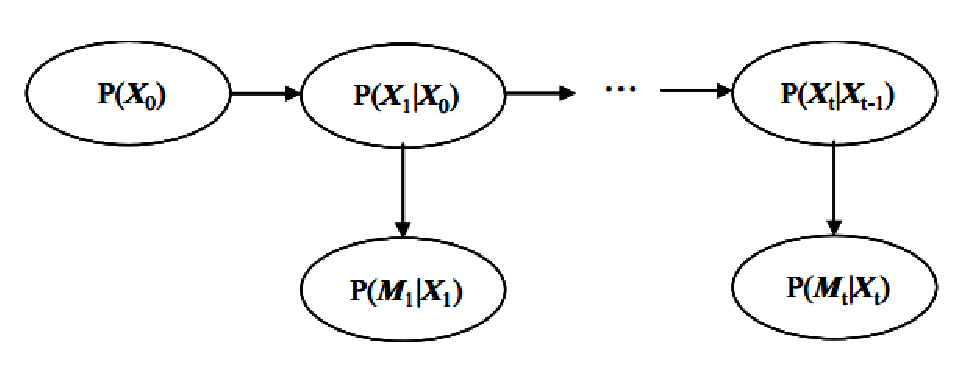
\includegraphics[width=0.7\textwidth]{dbn_bci}
\caption{Графическая модель сети для байесовского интервала правдоподобия (BCI)}
\label{fig:spec:DBN:BCI}
\end{figure}

Такая байесовская сеть отслеживает многомерные распределения линейных гауссовых переменных состояния и их наблюдаемые аналоги, которые измеряются с помощью датчиков. Скрытые переменные полагаются Марковскими процессами первого порядка, т.е. значение переменной в момент времени $t$ зависит только от состояния в момент времени $t-1$. Апостериорные вероятности скрытых и наблюдаемых переменных получаются с помощью фильтра Калмана, как только поступают новые измерения с датчиков. Данные вероятности используются для построения байесовского доверительного интервала $p\%$. Апостериорная вероятность $p$ отражает тот факт, что наблюдаемая переменная находится внутри интервала. Таким образом, любое измерение, попадающее за пределы доверительного интервала $p\%$, может быть классифицировано как аномалия~\cite{DBNAnomalyDetection}. Параметры сети (распределения вероятностей $P(X_0), P(X_t|X_{t-1}), P(M_t|X_t)$) могут быть получены из исходной выборки с помощью EM-алгоритма~\cite{KorolevEMAlgo}.

\subsubsection{Максимальная апостериорная оценка измерений (MAP-ms)}
В стратегии MAP-ms используется более сложная модель сети, показанная на рисунке~\ref{fig:spec:DBN:MAPms}. Векторы $X$ и $Z$ представляют непрерывные и дискретные скрытые переменные, а вектор $M$~---~наблюдаемые непрерывные переменные. Нижние индексы обозначают моменты времени.

\begin{figure}[h]
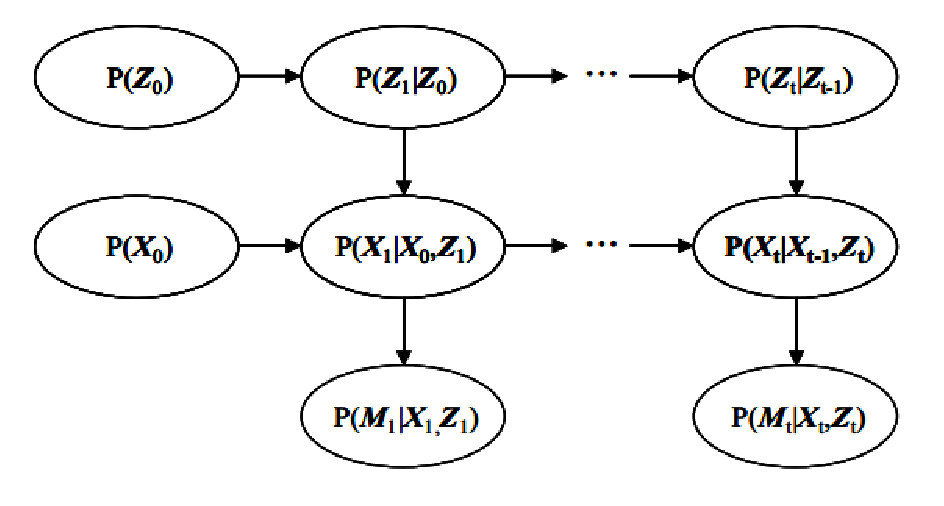
\includegraphics[width=0.7\textwidth]{dbn_mapms}
\caption{Графическая модель сети для максимального апостериорного статуса измерений (MAP-ms)}
\label{fig:spec:DBN:MAPms}
\end{figure}

Данная модель отслеживает многомерные многомерные распределения линейных гауссовых переменных состояния и их наблюдаемые аналоги, которые измеряются с помощью датчиков, как и вероятности скрытых дискретных переменных, показывающих статус каждого измерения (например, номинальный/аномальный). К примеру, если есть две измеряемых переменных состояния, то дискретная переменная статуса измерения будет иметь четыре возможных значения: (номинальный, номинальный), (аномальный, номинальный), (номинальный, аномальный) и (аномальный, аномальный). Апостериорные вероятности скрытых и наблюдаемых переменных получаются с помощью фильтра частиц Рао-Блэквелла, как только поступают новые измерения с датчиков. Максимальная апостериорная оценка измерения (например, наиболее вероятное значение, полученное из апостериорной вероятности) скрытой переменной состояния, показывающей статус измерения, может быть использована для классификации измерения как номинального или аномального. 

MAP-ms для работы требует, во-первых, параметры байесовской сети, описывающие изменение во времени линейных гауссовых переменных состояния для каждого значения дискретного статуса измерения, и, во-вторых, параметры, описывающие изменение во времени дискретных переменных. Кроме того, необходимо вручную задать вероятности для дискретных переменных ($P(Z_0), P(Z_t|Z_{t-1})$), опираясь на знание предметной области. Для случая, когда аномалий в исходной выборке нет, параметры сети совпадают с сетью для стратегии BCI, описанной в пункте~\ref{subsubsec:spec:DBN:BCI}. Если же одно или несколько измерений являются аномальными, параметры сети могут довольно сильно отличаться.~\cite{DBNAnomalyDetection}

Основные преимущества динамических байесовских сетей в применении к обнаружению аномалий:
\begin{itemize}
	\item способность работать в режиме реального времени~\cite{DBNAnomalyDetection};
	\item возможнсть графически представить модель системы.
\end{itemize}

Недостатки:
\begin{itemize}
	\item крайне высокая сложность метода;
	\item низкая эффективность на реальных данных~\cite{MartinCompUnsupervisedDetectionMethods}.
\end{itemize}